% Options for packages loaded elsewhere
\PassOptionsToPackage{unicode}{hyperref}
\PassOptionsToPackage{hyphens}{url}
%
\documentclass[
]{article}
\usepackage{amsmath,amssymb}
\usepackage{lmodern}
\usepackage{ifxetex,ifluatex}
\ifnum 0\ifxetex 1\fi\ifluatex 1\fi=0 % if pdftex
  \usepackage[T1]{fontenc}
  \usepackage[utf8]{inputenc}
  \usepackage{textcomp} % provide euro and other symbols
\else % if luatex or xetex
  \usepackage{unicode-math}
  \defaultfontfeatures{Scale=MatchLowercase}
  \defaultfontfeatures[\rmfamily]{Ligatures=TeX,Scale=1}
\fi
% Use upquote if available, for straight quotes in verbatim environments
\IfFileExists{upquote.sty}{\usepackage{upquote}}{}
\IfFileExists{microtype.sty}{% use microtype if available
  \usepackage[]{microtype}
  \UseMicrotypeSet[protrusion]{basicmath} % disable protrusion for tt fonts
}{}
\makeatletter
\@ifundefined{KOMAClassName}{% if non-KOMA class
  \IfFileExists{parskip.sty}{%
    \usepackage{parskip}
  }{% else
    \setlength{\parindent}{0pt}
    \setlength{\parskip}{6pt plus 2pt minus 1pt}}
}{% if KOMA class
  \KOMAoptions{parskip=half}}
\makeatother
\usepackage{xcolor}
\IfFileExists{xurl.sty}{\usepackage{xurl}}{} % add URL line breaks if available
\IfFileExists{bookmark.sty}{\usepackage{bookmark}}{\usepackage{hyperref}}
\hypersetup{
  pdftitle={Final Exam},
  hidelinks,
  pdfcreator={LaTeX via pandoc}}
\urlstyle{same} % disable monospaced font for URLs
\usepackage[margin=1in]{geometry}
\usepackage{color}
\usepackage{fancyvrb}
\newcommand{\VerbBar}{|}
\newcommand{\VERB}{\Verb[commandchars=\\\{\}]}
\DefineVerbatimEnvironment{Highlighting}{Verbatim}{commandchars=\\\{\}}
% Add ',fontsize=\small' for more characters per line
\usepackage{framed}
\definecolor{shadecolor}{RGB}{248,248,248}
\newenvironment{Shaded}{\begin{snugshade}}{\end{snugshade}}
\newcommand{\AlertTok}[1]{\textcolor[rgb]{0.94,0.16,0.16}{#1}}
\newcommand{\AnnotationTok}[1]{\textcolor[rgb]{0.56,0.35,0.01}{\textbf{\textit{#1}}}}
\newcommand{\AttributeTok}[1]{\textcolor[rgb]{0.77,0.63,0.00}{#1}}
\newcommand{\BaseNTok}[1]{\textcolor[rgb]{0.00,0.00,0.81}{#1}}
\newcommand{\BuiltInTok}[1]{#1}
\newcommand{\CharTok}[1]{\textcolor[rgb]{0.31,0.60,0.02}{#1}}
\newcommand{\CommentTok}[1]{\textcolor[rgb]{0.56,0.35,0.01}{\textit{#1}}}
\newcommand{\CommentVarTok}[1]{\textcolor[rgb]{0.56,0.35,0.01}{\textbf{\textit{#1}}}}
\newcommand{\ConstantTok}[1]{\textcolor[rgb]{0.00,0.00,0.00}{#1}}
\newcommand{\ControlFlowTok}[1]{\textcolor[rgb]{0.13,0.29,0.53}{\textbf{#1}}}
\newcommand{\DataTypeTok}[1]{\textcolor[rgb]{0.13,0.29,0.53}{#1}}
\newcommand{\DecValTok}[1]{\textcolor[rgb]{0.00,0.00,0.81}{#1}}
\newcommand{\DocumentationTok}[1]{\textcolor[rgb]{0.56,0.35,0.01}{\textbf{\textit{#1}}}}
\newcommand{\ErrorTok}[1]{\textcolor[rgb]{0.64,0.00,0.00}{\textbf{#1}}}
\newcommand{\ExtensionTok}[1]{#1}
\newcommand{\FloatTok}[1]{\textcolor[rgb]{0.00,0.00,0.81}{#1}}
\newcommand{\FunctionTok}[1]{\textcolor[rgb]{0.00,0.00,0.00}{#1}}
\newcommand{\ImportTok}[1]{#1}
\newcommand{\InformationTok}[1]{\textcolor[rgb]{0.56,0.35,0.01}{\textbf{\textit{#1}}}}
\newcommand{\KeywordTok}[1]{\textcolor[rgb]{0.13,0.29,0.53}{\textbf{#1}}}
\newcommand{\NormalTok}[1]{#1}
\newcommand{\OperatorTok}[1]{\textcolor[rgb]{0.81,0.36,0.00}{\textbf{#1}}}
\newcommand{\OtherTok}[1]{\textcolor[rgb]{0.56,0.35,0.01}{#1}}
\newcommand{\PreprocessorTok}[1]{\textcolor[rgb]{0.56,0.35,0.01}{\textit{#1}}}
\newcommand{\RegionMarkerTok}[1]{#1}
\newcommand{\SpecialCharTok}[1]{\textcolor[rgb]{0.00,0.00,0.00}{#1}}
\newcommand{\SpecialStringTok}[1]{\textcolor[rgb]{0.31,0.60,0.02}{#1}}
\newcommand{\StringTok}[1]{\textcolor[rgb]{0.31,0.60,0.02}{#1}}
\newcommand{\VariableTok}[1]{\textcolor[rgb]{0.00,0.00,0.00}{#1}}
\newcommand{\VerbatimStringTok}[1]{\textcolor[rgb]{0.31,0.60,0.02}{#1}}
\newcommand{\WarningTok}[1]{\textcolor[rgb]{0.56,0.35,0.01}{\textbf{\textit{#1}}}}
\usepackage{longtable,booktabs,array}
\usepackage{calc} % for calculating minipage widths
% Correct order of tables after \paragraph or \subparagraph
\usepackage{etoolbox}
\makeatletter
\patchcmd\longtable{\par}{\if@noskipsec\mbox{}\fi\par}{}{}
\makeatother
% Allow footnotes in longtable head/foot
\IfFileExists{footnotehyper.sty}{\usepackage{footnotehyper}}{\usepackage{footnote}}
\makesavenoteenv{longtable}
\usepackage{graphicx}
\makeatletter
\def\maxwidth{\ifdim\Gin@nat@width>\linewidth\linewidth\else\Gin@nat@width\fi}
\def\maxheight{\ifdim\Gin@nat@height>\textheight\textheight\else\Gin@nat@height\fi}
\makeatother
% Scale images if necessary, so that they will not overflow the page
% margins by default, and it is still possible to overwrite the defaults
% using explicit options in \includegraphics[width, height, ...]{}
\setkeys{Gin}{width=\maxwidth,height=\maxheight,keepaspectratio}
% Set default figure placement to htbp
\makeatletter
\def\fps@figure{htbp}
\makeatother
\setlength{\emergencystretch}{3em} % prevent overfull lines
\providecommand{\tightlist}{%
  \setlength{\itemsep}{0pt}\setlength{\parskip}{0pt}}
\setcounter{secnumdepth}{-\maxdimen} % remove section numbering
\ifluatex
  \usepackage{selnolig}  % disable illegal ligatures
\fi

\title{Final Exam}
\author{}
\date{\vspace{-2.5em}}

\begin{document}
\maketitle

\hypertarget{instructions}{%
\section{Instructions}\label{instructions}}

The final exam will be a one-on-one oral exam with the instructor.
Please meet the instructor near the ``fish-bowl'' office in the Data
Science Institute lobby. The exam will be recorded in Zoom. Please
prepare solutions to the following is a set of questions. During the
oral exam, the instructor will ask a series of questions covering topics
from the course and the questions. For example, the instructor may ask:

\begin{enumerate}
\def\labelenumi{\arabic{enumi}.}
\tightlist
\item
  Please explain how you solved a particular question.
\item
  Please solve a new question (perhaps closely related to a question
  below).
\item
  Please explain course topic X.
\end{enumerate}

You will be graded on both the accuracy of your responses and the
clarity with which you explain course concepts and solutions to
questions.

The final exam should represent your own work. Do not consult with or
collaborate in any way with anyone other than the instructor.

Prior to meeting with the instructor, you should:

\begin{itemize}
\tightlist
\item
  Create a folder in your Probability and Inference Portfolio; call it
  \texttt{99-final-exam}.
\item
  Compile, save, and push your solutions to your GitHub repository
\end{itemize}

\hypertarget{simulation}{%
\section{1. Simulation}\label{simulation}}

The Monte Hall problem is a classic game show. Contestants on the show
where shown three doors. Behind one randomly selected door was a
sportscar; behind the other doors were goats.

At the start of the game, contestants would select a door, say door A.
Then, the host would open either door B or C to reveal a goat. At that
point in the game, the host would ask the contestant if she would like
to change her door selection. Once a contestant decided to stay or
change, the host would open the chosen door to reveal the game prize,
either a goat or a car.

In this problem, consider a \textbf{modified} version of the Monte Hall
problem in which the number of doors is \textbf{variable}. Rather than 3
doors, consider a game with 4 or 5 or 50 doors. In the modified version
of the game, a contestant would select an initial door, say door A.
Then, the host would open \textbf{one} of the remaining doors to reveal
a goat. At that point in the game, the host would ask the contestant if
she would like to change her door selection. Once a contestant decided
to stay or change, the host would open the chosen door to reveal the
game prize, either a goat or a car.

Consider two strategies:

\begin{enumerate}
\def\labelenumi{\arabic{enumi}.}
\tightlist
\item
  Always stay with the first door selected.
\item
  Always switch to the unopened door.
\end{enumerate}

\textbf{C.} The function \texttt{game} below plays a single game of
Monte Hall. The function returns a vector of length two, the first
element is the prize under strategy 1 and the second element is the
prize under strategy 2. The function has a single input parameter, N,
which is the number of doors in the game.

Use the \texttt{game} function to estimate the probability that both
strategies result in a goat. Let \textbf{N=4}.

\begin{Shaded}
\begin{Highlighting}[]
\FunctionTok{require}\NormalTok{(magrittr)}
\end{Highlighting}
\end{Shaded}

\begin{verbatim}
## Loading required package: magrittr
\end{verbatim}

\begin{Shaded}
\begin{Highlighting}[]
\FunctionTok{require}\NormalTok{(dplyr)}
\end{Highlighting}
\end{Shaded}

\begin{verbatim}
## Loading required package: dplyr
\end{verbatim}

\begin{verbatim}
## 
## Attaching package: 'dplyr'
\end{verbatim}

\begin{verbatim}
## The following objects are masked from 'package:stats':
## 
##     filter, lag
\end{verbatim}

\begin{verbatim}
## The following objects are masked from 'package:base':
## 
##     intersect, setdiff, setequal, union
\end{verbatim}

\begin{Shaded}
\begin{Highlighting}[]
\NormalTok{game }\OtherTok{\textless{}{-}} \ControlFlowTok{function}\NormalTok{(N)\{}
  \ControlFlowTok{if}\NormalTok{(N}\SpecialCharTok{\textless{}}\DecValTok{3}\NormalTok{) }\FunctionTok{stop}\NormalTok{(}\StringTok{"Must have at least 3 doors"}\NormalTok{)}
\NormalTok{  prize }\OtherTok{\textless{}{-}} \FunctionTok{sample}\NormalTok{(}\FunctionTok{c}\NormalTok{(}\FunctionTok{rep}\NormalTok{(}\StringTok{"goat"}\NormalTok{,N}\DecValTok{{-}1}\NormalTok{),}\StringTok{"car"}\NormalTok{), N)}
\NormalTok{  guess }\OtherTok{\textless{}{-}} \FunctionTok{sample}\NormalTok{(}\DecValTok{1}\SpecialCharTok{:}\NormalTok{N,}\DecValTok{1}\NormalTok{)}
\NormalTok{  game }\OtherTok{\textless{}{-}} \FunctionTok{data.frame}\NormalTok{(}\AttributeTok{door =} \DecValTok{1}\SpecialCharTok{:}\NormalTok{N, }\AttributeTok{prize =}\NormalTok{ prize, }\AttributeTok{stringsAsFactors =} \ConstantTok{FALSE}\NormalTok{) }\SpecialCharTok{\%\textgreater{}\%} 
    \FunctionTok{mutate}\NormalTok{(}\AttributeTok{first\_guess =} \FunctionTok{case\_when}\NormalTok{(}
\NormalTok{      door }\SpecialCharTok{==}\NormalTok{ guess }\SpecialCharTok{\textasciitilde{}} \DecValTok{1}
\NormalTok{      , }\ConstantTok{TRUE} \SpecialCharTok{\textasciitilde{}} \DecValTok{0}
\NormalTok{    )) }\SpecialCharTok{\%\textgreater{}\%} 
    \FunctionTok{mutate}\NormalTok{(}\AttributeTok{potential\_reveal =} \FunctionTok{case\_when}\NormalTok{(}
\NormalTok{        first\_guess }\SpecialCharTok{==} \DecValTok{1} \SpecialCharTok{\textasciitilde{}} \DecValTok{0}
\NormalTok{      , prize }\SpecialCharTok{==} \StringTok{"car"} \SpecialCharTok{\textasciitilde{}} \DecValTok{0}
\NormalTok{      , }\ConstantTok{TRUE} \SpecialCharTok{\textasciitilde{}} \DecValTok{1}
\NormalTok{    )) }\SpecialCharTok{\%\textgreater{}\%} 
    \FunctionTok{mutate}\NormalTok{(}\AttributeTok{reveal =} \DecValTok{1}\SpecialCharTok{*}\NormalTok{(}\FunctionTok{rank}\NormalTok{(potential\_reveal, }\AttributeTok{ties.method =} \StringTok{"random"}\NormalTok{) }\SpecialCharTok{==} \DecValTok{3}\NormalTok{)) }\SpecialCharTok{\%\textgreater{}\%} 
    \FunctionTok{mutate}\NormalTok{(}\AttributeTok{potential\_switch =} \FunctionTok{case\_when}\NormalTok{(}
\NormalTok{      first\_guess }\SpecialCharTok{==} \DecValTok{1} \SpecialCharTok{\textasciitilde{}} \DecValTok{0}
\NormalTok{      , reveal }\SpecialCharTok{==} \DecValTok{1} \SpecialCharTok{\textasciitilde{}} \DecValTok{0}
\NormalTok{      , }\ConstantTok{TRUE} \SpecialCharTok{\textasciitilde{}} \DecValTok{1}
\NormalTok{    )) }\SpecialCharTok{\%\textgreater{}\%} 
    \FunctionTok{mutate}\NormalTok{(}\AttributeTok{switch =} \DecValTok{1}\SpecialCharTok{*}\NormalTok{(}\FunctionTok{rank}\NormalTok{(potential\_switch, }\AttributeTok{ties.method =} \StringTok{"random"}\NormalTok{) }\SpecialCharTok{==} \DecValTok{3}\NormalTok{))}
  \FunctionTok{c}\NormalTok{(game}\SpecialCharTok{$}\NormalTok{prize[game}\SpecialCharTok{$}\NormalTok{first\_guess }\SpecialCharTok{==} \DecValTok{1}\NormalTok{], game}\SpecialCharTok{$}\NormalTok{prize[game}\SpecialCharTok{$}\ControlFlowTok{switch} \SpecialCharTok{==} \DecValTok{1}\NormalTok{])}
\NormalTok{\}}
\end{Highlighting}
\end{Shaded}

\begin{Shaded}
\begin{Highlighting}[]
\DocumentationTok{\#\# p(win under strategy 1:stay with the first door selected)}
\NormalTok{(}\FunctionTok{rowMeans}\NormalTok{(}\FunctionTok{replicate}\NormalTok{(}\DecValTok{1000}\NormalTok{, }\FunctionTok{game}\NormalTok{(}\AttributeTok{N=}\DecValTok{4}\NormalTok{)) }\SpecialCharTok{==}\StringTok{"car"}\NormalTok{)[}\DecValTok{1}\NormalTok{])}
\end{Highlighting}
\end{Shaded}

\begin{verbatim}
## [1] 0.221
\end{verbatim}

\begin{Shaded}
\begin{Highlighting}[]
\DocumentationTok{\#\# p(win under strategy 1:switch door)}
\NormalTok{(}\FunctionTok{rowMeans}\NormalTok{(}\FunctionTok{replicate}\NormalTok{(}\DecValTok{1000}\NormalTok{, }\FunctionTok{game}\NormalTok{(}\AttributeTok{N=}\DecValTok{4}\NormalTok{)) }\SpecialCharTok{==}\StringTok{"car"}\NormalTok{)[}\DecValTok{2}\NormalTok{])}
\end{Highlighting}
\end{Shaded}

\begin{verbatim}
## [1] 0.371
\end{verbatim}

\textbf{B}. Communicate the precision of your simulated probability in
part \textbf{C} by calculating a \textbf{99\%} confidence interval.

\begin{Shaded}
\begin{Highlighting}[]
\CommentTok{\# strategy 1, wald confidence level}
\FunctionTok{prop.test}\NormalTok{(}\DecValTok{242}\NormalTok{,}\DecValTok{1000}\NormalTok{, }\AttributeTok{conf.level=}\FloatTok{0.99}\NormalTok{)}
\end{Highlighting}
\end{Shaded}

\begin{verbatim}
## 
##  1-sample proportions test with continuity correction
## 
## data:  242 out of 1000, null probability 0.5
## X-squared = 265.23, df = 1, p-value < 2.2e-16
## alternative hypothesis: true p is not equal to 0.5
## 99 percent confidence interval:
##  0.2084151 0.2790345
## sample estimates:
##     p 
## 0.242
\end{verbatim}

\begin{Shaded}
\begin{Highlighting}[]
\FunctionTok{prop.test}\NormalTok{(}\DecValTok{362}\NormalTok{,}\DecValTok{1000}\NormalTok{, }\AttributeTok{conf.level=}\FloatTok{0.99}\NormalTok{)}
\end{Highlighting}
\end{Shaded}

\begin{verbatim}
## 
##  1-sample proportions test with continuity correction
## 
## data:  362 out of 1000, null probability 0.5
## X-squared = 75.625, df = 1, p-value < 2.2e-16
## alternative hypothesis: true p is not equal to 0.5
## 99 percent confidence interval:
##  0.3233976 0.4024447
## sample estimates:
##     p 
## 0.362
\end{verbatim}

\textbf{A}. Let D(N) be the difference between the difference in
probabilities between strategy 2 and strategy 1.

\[
D(N) = P(\text{win strategy 2}|\text{N doors}) - P(\text{win strategy 1}|\text{N doors})
\] Create a plot that shows how D changes as N increases. Put N on the
x-asis, ranging from 3 to 10. Put D on the y-axis.

\begin{Shaded}
\begin{Highlighting}[]
\NormalTok{N }\OtherTok{\textless{}{-}} \FunctionTok{seq}\NormalTok{(}\DecValTok{3}\SpecialCharTok{:}\DecValTok{10}\NormalTok{)}
\NormalTok{y }\OtherTok{\textless{}{-}} \ConstantTok{NA}
\ControlFlowTok{for}\NormalTok{ (i }\ControlFlowTok{in}\NormalTok{ N)\{}
\NormalTok{  onegame }\OtherTok{\textless{}{-}} \FunctionTok{rowMeans}\NormalTok{(}\FunctionTok{replicate}\NormalTok{(}\DecValTok{1000}\NormalTok{, }\FunctionTok{game}\NormalTok{(}\AttributeTok{N=}\NormalTok{i}\SpecialCharTok{+}\DecValTok{2}\NormalTok{)) }\SpecialCharTok{==}\StringTok{"car"}\NormalTok{)}
\NormalTok{  y[i] }\OtherTok{\textless{}{-}}\NormalTok{ onegame[}\DecValTok{2}\NormalTok{]}\SpecialCharTok{{-}}\NormalTok{onegame[}\DecValTok{1}\NormalTok{]}
\NormalTok{\}}
\FunctionTok{plot}\NormalTok{(N,y)}
\end{Highlighting}
\end{Shaded}

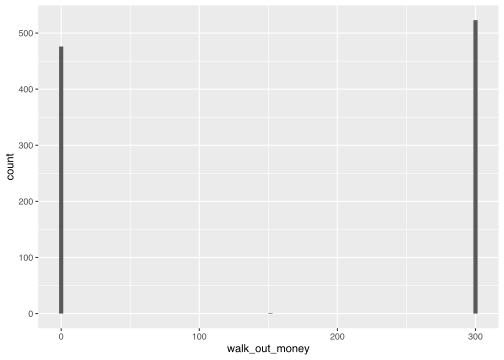
\includegraphics{Finalexam.Rmd_files/figure-latex/unnamed-chunk-4-1.pdf}

\hypertarget{probability}{%
\section{2. Probability}\label{probability}}

Consider a test for a rare genetic condition. Let T+ denote a test
result that indicates the condition is present, while T- denotes
absence. Let D+ and D- denote the true status of the disease.

\textbf{C}. Fill-in the probability table using the following
information:

\begin{itemize}
\tightlist
\item
  P(T+\textbar D+) = .85, and
\item
  P(T-\textbar D-) = .95, and
\item
  P(D+) = 0.001
\end{itemize}

\begin{longtable}[]{@{}cccc@{}}
\toprule
& D+ & D- & \\
\midrule
\endhead
T+ & & & \\
T- & & & \\
& 0.001 & & 1 \\
\bottomrule
\end{longtable}

\textbf{B}. Calculate the \textbf{negative} predictive value of the
test, P(D-\textbar T-).

\begin{Shaded}
\begin{Highlighting}[]
\CommentTok{\#conditional row probability = cell prob/row prob}
\NormalTok{(}\DecValTok{1}\FloatTok{{-}0.001}\NormalTok{)}\SpecialCharTok{*}\NormalTok{(}\FloatTok{0.95}\NormalTok{)}\SpecialCharTok{/}\NormalTok{((}\DecValTok{1}\FloatTok{{-}0.001}\NormalTok{)}\SpecialCharTok{*}\NormalTok{(}\FloatTok{0.95}\NormalTok{)}\SpecialCharTok{+}\FloatTok{0.001}\SpecialCharTok{*}\NormalTok{(}\DecValTok{1}\FloatTok{{-}0.85}\NormalTok{))}
\end{Highlighting}
\end{Shaded}

\begin{verbatim}
## [1] 0.999842
\end{verbatim}

\textbf{A} Create a plot that shows how the \textbf{positive} predictive
value as a function of the prevalence of disease, P(D+).

\begin{Shaded}
\begin{Highlighting}[]
\NormalTok{prevalence }\OtherTok{\textless{}{-}} \FunctionTok{seq}\NormalTok{(}\FloatTok{0.001}\NormalTok{, }\FloatTok{0.1}\NormalTok{, }\AttributeTok{length =} \DecValTok{50}\NormalTok{)}
\CommentTok{\#P(D+|T+)=(0.001*0.85)/((0.001*0.85)+((1{-}0.001)*(1{-}0.95))=0.0167}
\CommentTok{\#P(D+|T)}
\NormalTok{ppv }\OtherTok{\textless{}{-}}\NormalTok{ (prevalence}\SpecialCharTok{*}\FloatTok{0.85}\NormalTok{)}\SpecialCharTok{/}\NormalTok{((prevalence}\SpecialCharTok{*}\FloatTok{0.85}\NormalTok{)}\SpecialCharTok{+}\NormalTok{(}\DecValTok{1}\SpecialCharTok{{-}}\NormalTok{prevalence)}\SpecialCharTok{*}\NormalTok{(}\DecValTok{1}\FloatTok{{-}0.95}\NormalTok{))}
\FunctionTok{plot}\NormalTok{(prevalence, ppv, }\AttributeTok{xlab =} \StringTok{"Prevalence"}\NormalTok{, }\AttributeTok{ylab =} \StringTok{"PPV"}\NormalTok{,}\AttributeTok{type=}\StringTok{"l"}\NormalTok{)}
\end{Highlighting}
\end{Shaded}

\hypertarget{discrete-distributions}{%
\section{3. Discrete Distributions}\label{discrete-distributions}}

Suppose the yearly hospital charges (in thousands of dollars) for a
randomly selected Vanderbilt student is a mixture distribution.

For 50\% of students, the hospital charges will be \$0. For the
remaining 50\% of students, the hospital charges are a random variable
described by a gamma distribution with shape = 2 and scale = 2. (Again,
in thousands of dollars.)

\begin{Shaded}
\begin{Highlighting}[]
\NormalTok{hospital\_charges }\OtherTok{\textless{}{-}} \ControlFlowTok{function}\NormalTok{(N)\{}
\NormalTok{  group }\OtherTok{\textless{}{-}} \FunctionTok{rbinom}\NormalTok{(N, }\DecValTok{1}\NormalTok{, }\FloatTok{0.5}\NormalTok{)}
\NormalTok{  charges }\OtherTok{\textless{}{-}} \DecValTok{0}\SpecialCharTok{*}\NormalTok{group }\SpecialCharTok{+} \FunctionTok{rgamma}\NormalTok{(N, }\AttributeTok{shape =} \DecValTok{2}\NormalTok{, }\AttributeTok{scale =} \DecValTok{2}\NormalTok{)}\SpecialCharTok{*}\NormalTok{(}\DecValTok{1}\SpecialCharTok{{-}}\NormalTok{group)}
\NormalTok{  charges}
\NormalTok{\}}
\end{Highlighting}
\end{Shaded}

\textbf{C}. What is the 90th percentile for yearly hospital charges for
a randomly selected Vanderbilt student?

\begin{Shaded}
\begin{Highlighting}[]
\CommentTok{\#quantile(mean(replicate(10000, hospital\_charges(1))), 0.9)}
\end{Highlighting}
\end{Shaded}

\begin{Shaded}
\begin{Highlighting}[]
\FunctionTok{quantile}\NormalTok{(}\FunctionTok{replicate}\NormalTok{(}\DecValTok{10000}\NormalTok{, }\FunctionTok{hospital\_charges}\NormalTok{(}\DecValTok{1}\NormalTok{)), }\FloatTok{0.9}\NormalTok{)}
\end{Highlighting}
\end{Shaded}

\begin{verbatim}
##      90% 
## 5.943275
\end{verbatim}

\textbf{B}. Consider the \textbf{class} average yearly hospital charge
for the students in a class of size 30. Plot the density function or a
simulated histogram of the class average yearly hospital charge.

\begin{Shaded}
\begin{Highlighting}[]
\NormalTok{out }\OtherTok{\textless{}{-}} \ConstantTok{NA}
\NormalTok{x }\OtherTok{\textless{}{-}} \FunctionTok{seq}\NormalTok{(}\DecValTok{1}\SpecialCharTok{:}\DecValTok{10000}\NormalTok{)}
\ControlFlowTok{for}\NormalTok{ (i }\ControlFlowTok{in}\NormalTok{ x)\{}
\NormalTok{  out[i] }\OtherTok{\textless{}{-}} \FunctionTok{mean}\NormalTok{(}\FunctionTok{hospital\_charges}\NormalTok{(}\DecValTok{30}\NormalTok{))}
\NormalTok{\}}
\FunctionTok{hist}\NormalTok{(out,}\AttributeTok{freq=}\NormalTok{F)}
\end{Highlighting}
\end{Shaded}

\includegraphics{Finalexam.Rmd_files/figure-latex/unnamed-chunk-10-1.pdf}

\begin{Shaded}
\begin{Highlighting}[]
\CommentTok{\#curve()}
\end{Highlighting}
\end{Shaded}

\textbf{A}. What is the probability that a randomly selected class of
size 30 students will have less than 10 students with zero yearly
hospital charges?

\begin{Shaded}
\begin{Highlighting}[]
\CommentTok{\#rowMeans(replicate(1000, game(N=4)) =="car")[2]}
\NormalTok{out }\OtherTok{\textless{}{-}} \ConstantTok{NA}
\NormalTok{x }\OtherTok{\textless{}{-}} \FunctionTok{seq}\NormalTok{(}\DecValTok{1}\SpecialCharTok{:}\DecValTok{10000}\NormalTok{)}
\ControlFlowTok{for}\NormalTok{ (i }\ControlFlowTok{in}\NormalTok{ x)\{}
\NormalTok{  count}\OtherTok{=}\DecValTok{0}
  \ControlFlowTok{for}\NormalTok{ (x }\ControlFlowTok{in} \FunctionTok{hospital\_charges}\NormalTok{(}\DecValTok{30}\NormalTok{))\{}
    \ControlFlowTok{if}\NormalTok{ (x }\SpecialCharTok{==} \DecValTok{0}\NormalTok{)\{}
\NormalTok{      count }\OtherTok{=}\NormalTok{ count }\SpecialCharTok{+} \DecValTok{1}
\NormalTok{    \}}
\NormalTok{  \}}
  \ControlFlowTok{if}\NormalTok{ (count }\SpecialCharTok{\textless{}} \DecValTok{10}\NormalTok{)\{}
\NormalTok{    out[i]}\OtherTok{=} \DecValTok{1}
\NormalTok{  \}}
  \ControlFlowTok{else}\NormalTok{\{}
\NormalTok{    out[i] }\OtherTok{=} \DecValTok{0}
\NormalTok{  \}}
\NormalTok{\}}
\FunctionTok{sum}\NormalTok{(out)}\SpecialCharTok{/}\FunctionTok{length}\NormalTok{(out)}
\end{Highlighting}
\end{Shaded}

\begin{verbatim}
## [1] 0.0217
\end{verbatim}

\hypertarget{continuous-distributions}{%
\section{4. Continuous Distributions}\label{continuous-distributions}}

\textbf{C.} Suppose diastolic blood pressure (DBP) follows a normal
distribution with mean 80 mmHg and SD 15 mmHg. What is the probability
that a randomly sampled person’s DBP lies between 70 and 104 mmHg?

\begin{Shaded}
\begin{Highlighting}[]
\FunctionTok{pnorm}\NormalTok{(}\DecValTok{104}\NormalTok{,}\AttributeTok{mean=}\DecValTok{80}\NormalTok{, }\AttributeTok{sd=}\DecValTok{15}\NormalTok{)}\SpecialCharTok{{-}}\FunctionTok{pnorm}\NormalTok{(}\DecValTok{70}\NormalTok{,}\AttributeTok{mean=}\DecValTok{80}\NormalTok{, }\AttributeTok{sd=}\DecValTok{15}\NormalTok{)}
\end{Highlighting}
\end{Shaded}

\begin{verbatim}
## [1] 0.6927082
\end{verbatim}

\textbf{B.} Suppose a human femur was discovered that is 37 cm long.
Also suppose that using the NHANES data, researchers believe the
distribution of femur bones, by sex, are distributed as follows:

\begin{itemize}
\tightlist
\item
  Female adult femur \(\sim N(36, 3.3)\)
\item
  Male adult femur \(\sim N(40, 3.4)\)
\end{itemize}

\includegraphics{leg-length-distributions.svg}

Under the assumption that male and females are equally likely, what is
the probability that the discovered femur was from a male?

\begin{Shaded}
\begin{Highlighting}[]
\FloatTok{0.5}\SpecialCharTok{*}\FunctionTok{dnorm}\NormalTok{(}\DecValTok{37}\NormalTok{,}\AttributeTok{mean=}\DecValTok{40}\NormalTok{,}\AttributeTok{sd=}\FloatTok{3.4}\NormalTok{)}\SpecialCharTok{/}\NormalTok{(}\FloatTok{0.5}\SpecialCharTok{*}\FunctionTok{dnorm}\NormalTok{(}\DecValTok{37}\NormalTok{,}\AttributeTok{mean=}\DecValTok{36}\NormalTok{,}\AttributeTok{sd=}\FloatTok{3.3}\NormalTok{)}\SpecialCharTok{+}\FloatTok{0.5}\SpecialCharTok{*}\FunctionTok{dnorm}\NormalTok{(}\DecValTok{37}\NormalTok{,}\AttributeTok{mean=}\DecValTok{40}\NormalTok{, }\AttributeTok{sd=}\FloatTok{3.4}\NormalTok{))}
\end{Highlighting}
\end{Shaded}

\begin{verbatim}
## [1] 0.407765
\end{verbatim}

\textbf{A.} Continuing part \textbf{B}, generate a plot of P(femur from
male \textbar{} femur length = x). Let femur length range from 25 to 50.

\begin{Shaded}
\begin{Highlighting}[]
\NormalTok{femur\_length }\OtherTok{\textless{}{-}} \DecValTok{25}\SpecialCharTok{:}\DecValTok{50}
\NormalTok{prob\_male }\OtherTok{\textless{}{-}} \FunctionTok{dnorm}\NormalTok{(femur\_length,}\AttributeTok{mean=}\DecValTok{40}\NormalTok{,}\AttributeTok{sd=}\FloatTok{3.4}\NormalTok{)}\SpecialCharTok{/}\NormalTok{(}\FunctionTok{dnorm}\NormalTok{(femur\_length,}\AttributeTok{mean=}\DecValTok{36}\NormalTok{,}\AttributeTok{sd=}\FloatTok{3.3}\NormalTok{)}\SpecialCharTok{+}\FunctionTok{dnorm}\NormalTok{(femur\_length,}\AttributeTok{mean=}\DecValTok{40}\NormalTok{, }\AttributeTok{sd=}\FloatTok{3.4}\NormalTok{))}
\FunctionTok{plot.new}\NormalTok{()}
\FunctionTok{plot.window}\NormalTok{(}\AttributeTok{xlim =} \FunctionTok{c}\NormalTok{(}\DecValTok{25}\NormalTok{,}\DecValTok{50}\NormalTok{), }\AttributeTok{ylim =} \FunctionTok{c}\NormalTok{(}\DecValTok{0}\NormalTok{,}\DecValTok{1}\NormalTok{))}
\FunctionTok{lines}\NormalTok{(femur\_length, prob\_male)}
\FunctionTok{axis}\NormalTok{(}\DecValTok{1}\NormalTok{)}
\FunctionTok{axis}\NormalTok{(}\DecValTok{2}\NormalTok{)}
\FunctionTok{box}\NormalTok{()}
\FunctionTok{title}\NormalTok{(}\AttributeTok{xlab =} \StringTok{"Femur Length"}\NormalTok{, }\AttributeTok{ylab =} \StringTok{"P(Male | femur length)"}\NormalTok{)}
\end{Highlighting}
\end{Shaded}

\includegraphics{Finalexam.Rmd_files/figure-latex/unnamed-chunk-14-1.pdf}

\hypertarget{expectation-and-variance}{%
\section{5. Expectation and Variance}\label{expectation-and-variance}}

Let us revisit the yearly hospital charges distribution from a previous
section.

\begin{quote}
\textbf{Recall:} The yearly hospital charges (in thousands of dollars)
for a randomly selected Vanderbilt student is a mixture distribution.
For 50\% of students, the hospital charges will be \$0. For the
remaining 50\% of students, the hospital charges are a random variable
described by a gamma distribution with shape = 2 and scale = 2. (Again,
in thousands of dollars.)
\end{quote}

\begin{Shaded}
\begin{Highlighting}[]
\NormalTok{hospital\_charges }\OtherTok{\textless{}{-}} \ControlFlowTok{function}\NormalTok{(N)\{}
\NormalTok{  group }\OtherTok{\textless{}{-}} \FunctionTok{rbinom}\NormalTok{(N, }\DecValTok{1}\NormalTok{, }\FloatTok{0.5}\NormalTok{)}
\NormalTok{  charges }\OtherTok{\textless{}{-}} \DecValTok{0}\SpecialCharTok{*}\NormalTok{group }\SpecialCharTok{+} \FunctionTok{rgamma}\NormalTok{(N, }\AttributeTok{shape =} \DecValTok{2}\NormalTok{, }\AttributeTok{scale =} \DecValTok{2}\NormalTok{)}\SpecialCharTok{*}\NormalTok{(}\DecValTok{1}\SpecialCharTok{{-}}\NormalTok{group)}
\NormalTok{  charges}
\NormalTok{\}}
\end{Highlighting}
\end{Shaded}

\textbf{C.} What is E{[}yearly hospital charges{]}?

\begin{Shaded}
\begin{Highlighting}[]
\FunctionTok{mean}\NormalTok{(}\FunctionTok{hospital\_charges}\NormalTok{(}\DecValTok{100000}\NormalTok{))}
\end{Highlighting}
\end{Shaded}

\begin{verbatim}
## [1] 1.998109
\end{verbatim}

\textbf{B.} Suppose Vanderbilt implements a cap of \$10,000 on yearly
student hospital charges. What is the mean yearly hospital charge under
the new policy?

\begin{Shaded}
\begin{Highlighting}[]
\NormalTok{hospital\_charges\_cap }\OtherTok{\textless{}{-}} \ControlFlowTok{function}\NormalTok{(N)\{}
\NormalTok{  group }\OtherTok{\textless{}{-}} \FunctionTok{rbinom}\NormalTok{(N, }\DecValTok{1}\NormalTok{, }\FloatTok{0.5}\NormalTok{)}
\NormalTok{  charges }\OtherTok{\textless{}{-}} \DecValTok{0}\SpecialCharTok{*}\NormalTok{group }\SpecialCharTok{+} \FunctionTok{rgamma}\NormalTok{(N, }\AttributeTok{shape =} \DecValTok{2}\NormalTok{, }\AttributeTok{scale =} \DecValTok{2}\NormalTok{)}\SpecialCharTok{*}\NormalTok{(}\DecValTok{1}\SpecialCharTok{{-}}\NormalTok{group)}
  \ControlFlowTok{for}\NormalTok{ (i }\ControlFlowTok{in} \DecValTok{1}\SpecialCharTok{:}\FunctionTok{length}\NormalTok{(charges))\{}
    \ControlFlowTok{if}\NormalTok{ (charges[i]}\SpecialCharTok{\textgreater{}}\DecValTok{10}\NormalTok{)\{}
\NormalTok{      charges[i] }\OtherTok{=} \DecValTok{10}
\NormalTok{    \}}
\NormalTok{  \}}
\NormalTok{  charges}
\NormalTok{\}}

\FunctionTok{mean}\NormalTok{(}\FunctionTok{hospital\_charges\_cap}\NormalTok{(}\DecValTok{100000}\NormalTok{))}
\end{Highlighting}
\end{Shaded}

\begin{verbatim}
## [1] 1.954211
\end{verbatim}

\textbf{A.} What is the variance of yearly hospital charge under the new
policy?

\begin{Shaded}
\begin{Highlighting}[]
\FunctionTok{var}\NormalTok{(}\FunctionTok{hospital\_charges\_cap}\NormalTok{(}\DecValTok{100000}\NormalTok{))}
\end{Highlighting}
\end{Shaded}

\begin{verbatim}
## [1] 7.020907
\end{verbatim}

\hypertarget{transformations-sampling-distributions}{%
\section{6. Transformations \& Sampling
Distributions}\label{transformations-sampling-distributions}}

\textbf{C.} Consider the log normal distribution. If X is a log normal
random variable, then log(X) is a normal random variable. One way to
create pseudo-random draws from the log normal distribution is to
generate draws from a normal distribution and then to transform the
draws by exponentiating. The parameters of the log normal distribution
are the parameters of the underlying normal distribution, \(\mu\) and
\(\sigma\) (or \(\sigma^2\)).

Log normal data are prevalent is biological systems and econometrics.

Suppose a blood chemistry measure has a log normal distribution with
\(\mu\) = 0 and \(\sigma\) = 1. Generate an histogram or density curve
for the sampling distribution of the median when the sample size is 101.

\begin{Shaded}
\begin{Highlighting}[]
\NormalTok{out }\OtherTok{=} \ConstantTok{NA}
\NormalTok{x }\OtherTok{\textless{}{-}} \FunctionTok{seq}\NormalTok{(}\DecValTok{1}\SpecialCharTok{:}\DecValTok{10000}\NormalTok{)}
\ControlFlowTok{for}\NormalTok{ (i }\ControlFlowTok{in}\NormalTok{ x)\{}
\NormalTok{  out[i] }\OtherTok{\textless{}{-}} \FunctionTok{exp}\NormalTok{(}\FunctionTok{rnorm}\NormalTok{(}\DecValTok{101}\NormalTok{, }\AttributeTok{mean=}\DecValTok{0}\NormalTok{, }\AttributeTok{sd=}\DecValTok{1}\NormalTok{))}\SpecialCharTok{\%\textgreater{}\%}\NormalTok{ median}
\NormalTok{\}}
\FunctionTok{hist}\NormalTok{(out,}\AttributeTok{freq =} \ConstantTok{FALSE}\NormalTok{,}\AttributeTok{breaks =} \DecValTok{20}\NormalTok{)}
\FunctionTok{lines}\NormalTok{(}\FunctionTok{density}\NormalTok{(out),}\AttributeTok{lty=}\DecValTok{2}\NormalTok{,}\AttributeTok{lwd=}\DecValTok{3}\NormalTok{,}\AttributeTok{col=}\StringTok{"steelblue"}\NormalTok{)}
\end{Highlighting}
\end{Shaded}

\includegraphics{Finalexam.Rmd_files/figure-latex/unnamed-chunk-19-1.pdf}

\textbf{B.} Below is the CDF function for the kth order statistic when
the underlying distribution is log normal with \(\mu\) = 0 and
\(\sigma\) = 1. Create a plot of the ECDF of the simulated sampling
distribution generated in \textbf{C} and overlay the CDF using the
function below.

\begin{Shaded}
\begin{Highlighting}[]
\NormalTok{Fk }\OtherTok{\textless{}{-}} \ControlFlowTok{function}\NormalTok{(x,k,n)\{}
  \FunctionTok{pbinom}\NormalTok{(k}\DecValTok{{-}1}\NormalTok{, n, }\FunctionTok{plnorm}\NormalTok{(x), }\AttributeTok{lower.tail =} \ConstantTok{FALSE}\NormalTok{)}
\NormalTok{\}}
\FunctionTok{plot}\NormalTok{(}\FunctionTok{ecdf}\NormalTok{(out),}\AttributeTok{lwd=}\DecValTok{3}\NormalTok{)}
\FunctionTok{curve}\NormalTok{(}\FunctionTok{Fk}\NormalTok{(x,}\AttributeTok{k=}\DecValTok{51}\NormalTok{,}\AttributeTok{n=}\DecValTok{101}\NormalTok{),}\AttributeTok{add=}\ConstantTok{TRUE}\NormalTok{,}\AttributeTok{col=}\StringTok{"blue"}\NormalTok{)}
\end{Highlighting}
\end{Shaded}

\includegraphics{Finalexam.Rmd_files/figure-latex/unnamed-chunk-20-1.pdf}

\textbf{A.} Of the 25th, 50th, and 75th quantiles of the distribution
from \textbf{B}, which will have the tightest 95\% CI? (Show the
sampling distribution of each.

\begin{Shaded}
\begin{Highlighting}[]
\NormalTok{dorder }\OtherTok{\textless{}{-}} \ControlFlowTok{function}\NormalTok{(x, k, n)\{}
\NormalTok{  k}\SpecialCharTok{*}\FunctionTok{choose}\NormalTok{(n,k)}\SpecialCharTok{*}
\NormalTok{    (}\FunctionTok{plnorm}\NormalTok{(x,}\DecValTok{0}\NormalTok{,}\DecValTok{1}\NormalTok{))}\SpecialCharTok{\^{}}\NormalTok{(k}\DecValTok{{-}1}\NormalTok{)}\SpecialCharTok{*}
\NormalTok{    (}\DecValTok{1}\SpecialCharTok{{-}}\FunctionTok{plnorm}\NormalTok{(x,}\DecValTok{0}\NormalTok{,}\DecValTok{1}\NormalTok{))}\SpecialCharTok{\^{}}\NormalTok{(n}\SpecialCharTok{{-}}\NormalTok{k)}\SpecialCharTok{*}
    \FunctionTok{dlnorm}\NormalTok{(x,}\DecValTok{0}\NormalTok{,}\DecValTok{1}\NormalTok{)}
\NormalTok{\}}

\FunctionTok{curve}\NormalTok{(}\FunctionTok{dorder}\NormalTok{(x, }\DecValTok{26}\NormalTok{, }\DecValTok{101}\NormalTok{), }\DecValTok{0}\NormalTok{,}\DecValTok{3}\NormalTok{,}\AttributeTok{ylab=}\StringTok{"Density"}\NormalTok{)}
\FunctionTok{curve}\NormalTok{(}\FunctionTok{dorder}\NormalTok{(x, }\DecValTok{51}\NormalTok{, }\DecValTok{101}\NormalTok{), }\AttributeTok{ylab=}\StringTok{"Density"}\NormalTok{,}\AttributeTok{col=}\StringTok{"green"}\NormalTok{,}\AttributeTok{add=} \ConstantTok{TRUE}\NormalTok{)}
\FunctionTok{curve}\NormalTok{(}\FunctionTok{dorder}\NormalTok{(x, }\DecValTok{76}\NormalTok{, }\DecValTok{101}\NormalTok{), }\AttributeTok{ylab=}\StringTok{"Density"}\NormalTok{,}\AttributeTok{add=} \ConstantTok{TRUE}\NormalTok{,}\AttributeTok{col=}\StringTok{"red"}\NormalTok{)}
\end{Highlighting}
\end{Shaded}

\includegraphics{Finalexam.Rmd_files/figure-latex/unnamed-chunk-21-1.pdf}

\begin{Shaded}
\begin{Highlighting}[]
\FunctionTok{curve}\NormalTok{(}\FunctionTok{Fk}\NormalTok{(x, }\DecValTok{26}\NormalTok{, }\DecValTok{101}\NormalTok{), }\DecValTok{0}\NormalTok{,}\DecValTok{3}\NormalTok{,}\AttributeTok{ylab=}\StringTok{"Density"}\NormalTok{)}
\FunctionTok{curve}\NormalTok{(}\FunctionTok{Fk}\NormalTok{(x, }\DecValTok{51}\NormalTok{, }\DecValTok{101}\NormalTok{), }\AttributeTok{ylab=}\StringTok{"Density"}\NormalTok{,}\AttributeTok{col=}\StringTok{"green"}\NormalTok{,}\AttributeTok{add=} \ConstantTok{TRUE}\NormalTok{)}
\FunctionTok{curve}\NormalTok{(}\FunctionTok{Fk}\NormalTok{(x, }\DecValTok{76}\NormalTok{, }\DecValTok{101}\NormalTok{), }\AttributeTok{ylab=}\StringTok{"Density"}\NormalTok{,}\AttributeTok{add=} \ConstantTok{TRUE}\NormalTok{,}\AttributeTok{col=}\StringTok{"red"}\NormalTok{)}
\end{Highlighting}
\end{Shaded}

\includegraphics{Finalexam.Rmd_files/figure-latex/unnamed-chunk-22-1.pdf}

\begin{Shaded}
\begin{Highlighting}[]
\CommentTok{\# So 25th quantiles has the tightest 95\% CI}
\end{Highlighting}
\end{Shaded}

\hypertarget{estimation-of-cdf-and-pdf-from-data}{%
\section{7. Estimation of CDF and PDF from
data}\label{estimation-of-cdf-and-pdf-from-data}}

The following code will load the NHANES data and select the first 500
rows.

\begin{Shaded}
\begin{Highlighting}[]
\NormalTok{Hmisc}\SpecialCharTok{::}\FunctionTok{getHdata}\NormalTok{(nhgh)}
\NormalTok{d1 }\OtherTok{\textless{}{-}}\NormalTok{ nhgh[}\DecValTok{1}\SpecialCharTok{:}\DecValTok{500}\NormalTok{,]}
\end{Highlighting}
\end{Shaded}

\textbf{C.} Estimate the distribution of standing height for adult (age
\textgreater{} 18) males using the MLE method with a normal
distribution. Create a plot of the estimated density function.

\begin{Shaded}
\begin{Highlighting}[]
\NormalTok{d2 }\OtherTok{\textless{}{-}}\NormalTok{ d1 }\SpecialCharTok{\%\textgreater{}\%} 
  \FunctionTok{filter}\NormalTok{(sex}\SpecialCharTok{==}\StringTok{"male"}\NormalTok{) }\SpecialCharTok{\%\textgreater{}\%} 
  \FunctionTok{filter}\NormalTok{(age }\SpecialCharTok{\textgreater{}=} \DecValTok{18}\NormalTok{) }\SpecialCharTok{\%\textgreater{}\%} 
  \FunctionTok{filter}\NormalTok{(}\FunctionTok{complete.cases}\NormalTok{(ht)) }\SpecialCharTok{\%\textgreater{}\%} 
  \FunctionTok{pull}\NormalTok{(ht)}


\FunctionTok{require}\NormalTok{(stats4)}
\end{Highlighting}
\end{Shaded}

\begin{verbatim}
## Loading required package: stats4
\end{verbatim}

\begin{Shaded}
\begin{Highlighting}[]
\NormalTok{nLL }\OtherTok{\textless{}{-}} \ControlFlowTok{function}\NormalTok{(mean, sd)\{}
\NormalTok{  fs }\OtherTok{\textless{}{-}} \FunctionTok{dnorm}\NormalTok{(}
        \AttributeTok{x =}\NormalTok{ d2}
\NormalTok{      , }\AttributeTok{mean =}\NormalTok{ mean}
\NormalTok{      , }\AttributeTok{sd =}\NormalTok{ sd}
\NormalTok{      , }\AttributeTok{log =} \ConstantTok{TRUE}
\NormalTok{    ) }
  \SpecialCharTok{{-}}\FunctionTok{sum}\NormalTok{(fs)}
\NormalTok{\}}
\NormalTok{fit }\OtherTok{\textless{}{-}} \FunctionTok{mle}\NormalTok{(}
\NormalTok{    nLL}
\NormalTok{  , }\AttributeTok{start =} \FunctionTok{list}\NormalTok{(}\AttributeTok{mean =} \DecValTok{1}\NormalTok{, }\AttributeTok{sd =} \DecValTok{1}\NormalTok{)}
\NormalTok{  , }\AttributeTok{method =} \StringTok{"L{-}BFGS{-}B"}
\NormalTok{  , }\AttributeTok{lower =} \FunctionTok{c}\NormalTok{(}\DecValTok{0}\NormalTok{, }\FloatTok{0.01}\NormalTok{)}
\NormalTok{)}
\NormalTok{mean\_hat}\OtherTok{=}\FunctionTok{coef}\NormalTok{(fit)[}\DecValTok{1}\NormalTok{]}
\NormalTok{sd\_hat}\OtherTok{=}\FunctionTok{coef}\NormalTok{(fit)[}\DecValTok{2}\NormalTok{]}

\FunctionTok{hist}\NormalTok{(d2,}\AttributeTok{freq=}\ConstantTok{FALSE}\NormalTok{)}
\FunctionTok{curve}\NormalTok{(}\FunctionTok{dnorm}\NormalTok{(x,mean\_hat, sd\_hat),}\AttributeTok{add=}\ConstantTok{TRUE}\NormalTok{)}
\end{Highlighting}
\end{Shaded}

\includegraphics{Finalexam.Rmd_files/figure-latex/unnamed-chunk-24-1.pdf}

\textbf{B.} Estimate the distribution of BMI for adult (age
\textgreater{} 18) females using using the method of moment method with
the gamma distribution. Create a plot of the estimated density function.

\begin{Shaded}
\begin{Highlighting}[]
\NormalTok{d3 }\OtherTok{\textless{}{-}}\NormalTok{ d1 }\SpecialCharTok{\%\textgreater{}\%} 
  \FunctionTok{filter}\NormalTok{(sex}\SpecialCharTok{==}\StringTok{"female"}\NormalTok{) }\SpecialCharTok{\%\textgreater{}\%} 
  \FunctionTok{filter}\NormalTok{(age }\SpecialCharTok{\textgreater{}=} \DecValTok{18}\NormalTok{) }\SpecialCharTok{\%\textgreater{}\%} 
  \FunctionTok{filter}\NormalTok{(}\FunctionTok{complete.cases}\NormalTok{(bmi)) }\SpecialCharTok{\%\textgreater{}\%} 
  \FunctionTok{pull}\NormalTok{(bmi)}

\FunctionTok{hist}\NormalTok{(d3, }\AttributeTok{freq =} \ConstantTok{FALSE}\NormalTok{, }\AttributeTok{main =} \StringTok{""}\NormalTok{)}
\CommentTok{\#parameters}
\NormalTok{(xbar }\OtherTok{\textless{}{-}} \FunctionTok{mean}\NormalTok{(d3))}
\end{Highlighting}
\end{Shaded}

\begin{verbatim}
## [1] 29.29143
\end{verbatim}

\begin{Shaded}
\begin{Highlighting}[]
\NormalTok{(s2 }\OtherTok{\textless{}{-}} \FunctionTok{var}\NormalTok{(d3))}
\end{Highlighting}
\end{Shaded}

\begin{verbatim}
## [1] 57.7764
\end{verbatim}

\begin{Shaded}
\begin{Highlighting}[]
\NormalTok{(shape\_hat }\OtherTok{\textless{}{-}}\NormalTok{ xbar}\SpecialCharTok{\^{}}\DecValTok{2}\SpecialCharTok{/}\NormalTok{s2)}
\end{Highlighting}
\end{Shaded}

\begin{verbatim}
## [1] 14.85015
\end{verbatim}

\begin{Shaded}
\begin{Highlighting}[]
\NormalTok{(scale\_hat }\OtherTok{\textless{}{-}}\NormalTok{ s2}\SpecialCharTok{/}\NormalTok{xbar)}
\end{Highlighting}
\end{Shaded}

\begin{verbatim}
## [1] 1.972467
\end{verbatim}

\begin{Shaded}
\begin{Highlighting}[]
\CommentTok{\#est pdf}
\FunctionTok{curve}\NormalTok{(}\FunctionTok{dgamma}\NormalTok{(x, }\AttributeTok{shape=}\NormalTok{shape\_hat, }\AttributeTok{scale=}\NormalTok{scale\_hat),}\AttributeTok{add =}\NormalTok{T,}\AttributeTok{lwd=}\DecValTok{3}\NormalTok{, }\AttributeTok{col=}\StringTok{"purple"}\NormalTok{)}
\end{Highlighting}
\end{Shaded}

\includegraphics{Finalexam.Rmd_files/figure-latex/unnamed-chunk-25-1.pdf}

\textbf{A.} Estimate the distribution of creatinine (SCr) for adults
(age \textgreater{} 18) using the kernel density method with a Gaussian
kernel. Create a plot of the estimated density function.

\begin{Shaded}
\begin{Highlighting}[]
\NormalTok{d4 }\OtherTok{\textless{}{-}}\NormalTok{ d1 }\SpecialCharTok{\%\textgreater{}\%} 
  \FunctionTok{filter}\NormalTok{(age }\SpecialCharTok{\textgreater{}=} \DecValTok{18}\NormalTok{) }\SpecialCharTok{\%\textgreater{}\%} 
  \FunctionTok{filter}\NormalTok{(}\FunctionTok{complete.cases}\NormalTok{(SCr)) }\SpecialCharTok{\%\textgreater{}\%} 
  \FunctionTok{pull}\NormalTok{(SCr)}

\NormalTok{epdfstar }\OtherTok{\textless{}{-}} \ControlFlowTok{function}\NormalTok{(t, data, smooth)\{}
  \FunctionTok{outer}\NormalTok{(t, data, }\ControlFlowTok{function}\NormalTok{(a,b)\{ }\FunctionTok{dnorm}\NormalTok{(a, b, smooth)\}) }\SpecialCharTok{\%\textgreater{}\%}\NormalTok{ rowMeans}
\NormalTok{\}}
\FunctionTok{hist}\NormalTok{(d4, }\AttributeTok{xlim =} \FunctionTok{c}\NormalTok{(}\SpecialCharTok{{-}}\DecValTok{2}\NormalTok{,}\DecValTok{5}\NormalTok{),}\AttributeTok{freq =} \ConstantTok{FALSE}\NormalTok{, }\AttributeTok{main =} \StringTok{""}\NormalTok{)}
\FunctionTok{curve}\NormalTok{(}\FunctionTok{epdfstar}\NormalTok{(x, d4, }\AttributeTok{smooth =} \FloatTok{0.5}\NormalTok{), }\AttributeTok{add =} \ConstantTok{TRUE}\NormalTok{, }\AttributeTok{lwd =} \DecValTok{3}\NormalTok{, }\AttributeTok{col =} \StringTok{"blue"}\NormalTok{)}
\FunctionTok{curve}\NormalTok{(}\FunctionTok{epdfstar}\NormalTok{(x, d4, }\AttributeTok{smooth =} \DecValTok{1}\NormalTok{), }\AttributeTok{add =} \ConstantTok{TRUE}\NormalTok{, }\AttributeTok{lwd =} \DecValTok{3}\NormalTok{, }\AttributeTok{col =} \StringTok{"black"}\NormalTok{)}
\end{Highlighting}
\end{Shaded}

\includegraphics{Finalexam.Rmd_files/figure-latex/unnamed-chunk-26-1.pdf}

\begin{Shaded}
\begin{Highlighting}[]
\CommentTok{\# I prefer smooth = 0.5, for it capture more variance in the data.}
\end{Highlighting}
\end{Shaded}

\hypertarget{sample-from-an-estimated-distribution}{%
\section{8. Sample from an estimated
distribution}\label{sample-from-an-estimated-distribution}}

The following code will load the low birth weight data from the MASS
package. The description of the variables in the dataset can be found in
the birthwt documentation with the command \texttt{?MASS::birthwt}.

\begin{Shaded}
\begin{Highlighting}[]
\NormalTok{bwt }\OtherTok{\textless{}{-}}\NormalTok{ MASS}\SpecialCharTok{::}\NormalTok{birthwt}
\end{Highlighting}
\end{Shaded}

\textbf{C.} Generate a 95\% confidence interval for the mean birthweight
of infants whose mothers \textbf{did} smoke during pregnancy using the
bootstrap.

\begin{Shaded}
\begin{Highlighting}[]
\NormalTok{bw }\OtherTok{\textless{}{-}}\NormalTok{ bwt }\SpecialCharTok{\%\textgreater{}\%} 
  \FunctionTok{filter}\NormalTok{(smoke}\SpecialCharTok{==}\DecValTok{1}\NormalTok{) }\SpecialCharTok{\%\textgreater{}\%}
  \FunctionTok{pull}\NormalTok{(bwt)}

\NormalTok{l }\OtherTok{\textless{}{-}} \FunctionTok{length}\NormalTok{(bw)}
\NormalTok{M}\OtherTok{\textless{}{-}} \DecValTok{5000}
\NormalTok{out }\OtherTok{\textless{}{-}} \ConstantTok{NA}
\ControlFlowTok{for}\NormalTok{ (i }\ControlFlowTok{in} \DecValTok{1}\SpecialCharTok{:}\NormalTok{M)\{}
\NormalTok{  index }\OtherTok{\textless{}{-}} \FunctionTok{sample.int}\NormalTok{(l,l,}\AttributeTok{replace =}\NormalTok{ T)}
\NormalTok{  out[i] }\OtherTok{\textless{}{-}} \FunctionTok{mean}\NormalTok{(bw[index])}
\NormalTok{\}}
\NormalTok{alpha}\OtherTok{\textless{}{-}} \FloatTok{0.05}
\FunctionTok{quantile}\NormalTok{(out,}\FunctionTok{c}\NormalTok{(}\FloatTok{0.025}\NormalTok{, }\FloatTok{0.975}\NormalTok{))}
\end{Highlighting}
\end{Shaded}

\begin{verbatim}
##     2.5%    97.5% 
## 2623.916 2915.009
\end{verbatim}

\textbf{B.} Generate a 95\% confidence interval for the mean birthweight
of infants whose mothers \textbf{did} smoke during pregnancy using the
Central Limit Theorem shortcut.

\begin{Shaded}
\begin{Highlighting}[]
\FunctionTok{t.test}\NormalTok{(bw)}
\end{Highlighting}
\end{Shaded}

\begin{verbatim}
## 
##  One Sample t-test
## 
## data:  bw
## t = 36.149, df = 73, p-value < 2.2e-16
## alternative hypothesis: true mean is not equal to 0
## 95 percent confidence interval:
##  2619.094 2924.744
## sample estimates:
## mean of x 
##  2771.919
\end{verbatim}

\textbf{A.} Let \(\mu_s\) be the mean birthweight of infants whose
mothers smoked during pregnancy. Let \(\mu_{ns}\) be the mean for the
non-smoking group. Use simulation to calculate the 95\% confidence
interval for \(\mu_s/\mu_{ns}\).

\begin{Shaded}
\begin{Highlighting}[]
\NormalTok{nos }\OtherTok{\textless{}{-}}\NormalTok{ bwt }\SpecialCharTok{\%\textgreater{}\%} 
  \FunctionTok{filter}\NormalTok{(smoke}\SpecialCharTok{==}\DecValTok{0}\NormalTok{) }\SpecialCharTok{\%\textgreater{}\%}
  \FunctionTok{pull}\NormalTok{(bwt)}
\NormalTok{R }\OtherTok{\textless{}{-}} \DecValTok{5000}
\NormalTok{means }\OtherTok{\textless{}{-}} \FunctionTok{rep}\NormalTok{(}\ConstantTok{NA}\NormalTok{, R)}
\NormalTok{mean\_smoke }\OtherTok{\textless{}{-}} \FunctionTok{mean}\NormalTok{(bw, }\AttributeTok{na.rm =} \ConstantTok{TRUE}\NormalTok{)}
\NormalTok{sd\_smoke }\OtherTok{\textless{}{-}} \FunctionTok{sd}\NormalTok{(bw, }\AttributeTok{na.rm =} \ConstantTok{TRUE}\NormalTok{)}

\NormalTok{mean\_no }\OtherTok{\textless{}{-}} \FunctionTok{mean}\NormalTok{(nos, }\AttributeTok{na.rm =} \ConstantTok{TRUE}\NormalTok{)}
\NormalTok{sd\_no }\OtherTok{\textless{}{-}}\FunctionTok{sd}\NormalTok{(nos, }\AttributeTok{na.rm =} \ConstantTok{TRUE}\NormalTok{)}
\ControlFlowTok{for}\NormalTok{(i }\ControlFlowTok{in} \DecValTok{1}\SpecialCharTok{:}\NormalTok{R)\{}
\NormalTok{  s }\OtherTok{\textless{}{-}} \FunctionTok{rnorm}\NormalTok{(}\FunctionTok{length}\NormalTok{(bwt), }\AttributeTok{mean =}\NormalTok{ mean\_smoke, }\AttributeTok{sd =}\NormalTok{ sd\_smoke)}
\NormalTok{  y }\OtherTok{\textless{}{-}} \FunctionTok{rnorm}\NormalTok{(}\FunctionTok{length}\NormalTok{(bwt), }\AttributeTok{mean =}\NormalTok{ mean\_no, }\AttributeTok{sd =}\NormalTok{ sd\_no)}
\NormalTok{  means[i] }\OtherTok{\textless{}{-}} \FunctionTok{mean}\NormalTok{(s)}\SpecialCharTok{/}\FunctionTok{mean}\NormalTok{(y)}
\NormalTok{\}}
\NormalTok{alpha }\OtherTok{\textless{}{-}} \FloatTok{0.05}
\NormalTok{t0 }\OtherTok{\textless{}{-}} \FunctionTok{quantile}\NormalTok{(means, }\FunctionTok{c}\NormalTok{(alpha}\SpecialCharTok{/}\DecValTok{2}\NormalTok{, }\DecValTok{1}\SpecialCharTok{{-}}\NormalTok{alpha}\SpecialCharTok{/}\DecValTok{2}\NormalTok{))}
\NormalTok{t0}
\end{Highlighting}
\end{Shaded}

\begin{verbatim}
##      2.5%     97.5% 
## 0.7334333 1.1271764
\end{verbatim}

\hypertarget{inference}{%
\section{9. Inference}\label{inference}}

\textbf{C.} Suppose two studies were performed looking at the risk of
mild complication after hernia repair using open and laparoscopic
surgical approaches. The study results are below. Using the data from
each study individually, perform the hypothesis test that the risk of
complication between open and laparoscopic repairs are the same under
the usual point null. What is the p-value from each study? What do you
conclude from each study?

\begin{Shaded}
\begin{Highlighting}[]
\FunctionTok{prop.test}\NormalTok{(}\AttributeTok{x=}\FunctionTok{c}\NormalTok{(}\DecValTok{30}\NormalTok{,}\DecValTok{35}\NormalTok{),}\AttributeTok{n=}\FunctionTok{c}\NormalTok{(}\DecValTok{100}\NormalTok{,}\DecValTok{100}\NormalTok{))}
\end{Highlighting}
\end{Shaded}

\begin{verbatim}
## 
##  2-sample test for equality of proportions with continuity correction
## 
## data:  c(30, 35) out of c(100, 100)
## X-squared = 0.36467, df = 1, p-value = 0.5459
## alternative hypothesis: two.sided
## 95 percent confidence interval:
##  -0.18963943  0.08963943
## sample estimates:
## prop 1 prop 2 
##   0.30   0.35
\end{verbatim}

\begin{Shaded}
\begin{Highlighting}[]
\CommentTok{\# p is 0.5459, if null,the risk of complication between open and laparoscopic repairs are the same, is true, the probabbilithy of us observe data in this study is 0.5459. We do not have evidence against the null.}
\end{Highlighting}
\end{Shaded}

\begin{Shaded}
\begin{Highlighting}[]
\FunctionTok{prop.test}\NormalTok{(}\AttributeTok{x=}\FunctionTok{c}\NormalTok{(}\DecValTok{600}\NormalTok{,}\DecValTok{619}\NormalTok{),}\AttributeTok{n=}\FunctionTok{c}\NormalTok{(}\DecValTok{1000}\NormalTok{,}\DecValTok{1000}\NormalTok{))}
\end{Highlighting}
\end{Shaded}

\begin{verbatim}
## 
##  2-sample test for equality of proportions with continuity correction
## 
## data:  c(600, 619) out of c(1000, 1000)
## X-squared = 0.68064, df = 1, p-value = 0.4094
## alternative hypothesis: two.sided
## 95 percent confidence interval:
##  -0.06275413  0.02475413
## sample estimates:
## prop 1 prop 2 
##  0.600  0.619
\end{verbatim}

\begin{Shaded}
\begin{Highlighting}[]
\CommentTok{\# p is 0.4094, if null,the risk of complication between open and laparoscopic repairs are the same, is true, the probabbilithy of us observe data in this study is 0.4094. We do not have evidence against the null.}
\end{Highlighting}
\end{Shaded}

\begin{longtable}[]{@{}lll@{}}
\toprule
Study 1 & Comp & No comp \\
\midrule
\endhead
Open & 30 & 70 \\
Lap & 35 & 65 \\
\bottomrule
\end{longtable}

\begin{longtable}[]{@{}lll@{}}
\toprule
Study 2 & Comp & No comp \\
\midrule
\endhead
Open & 600 & 1400 \\
Lap & 619 & 1381 \\
\bottomrule
\end{longtable}

\textbf{B.} Suppose that prior to the studies, the researchers
established an equivalence threshold of 6 percentage points. Using the
confidence intervals, which studies (if any) showed a conclusive
similarity between surgical approaches for the complication rate.
Explain why.

\begin{Shaded}
\begin{Highlighting}[]
\FunctionTok{prop.test}\NormalTok{(}\AttributeTok{x=}\FunctionTok{c}\NormalTok{(}\DecValTok{30}\NormalTok{,}\DecValTok{35}\NormalTok{),}\AttributeTok{n=}\FunctionTok{c}\NormalTok{(}\DecValTok{100}\NormalTok{,}\DecValTok{100}\NormalTok{))}
\end{Highlighting}
\end{Shaded}

\begin{verbatim}
## 
##  2-sample test for equality of proportions with continuity correction
## 
## data:  c(30, 35) out of c(100, 100)
## X-squared = 0.36467, df = 1, p-value = 0.5459
## alternative hypothesis: two.sided
## 95 percent confidence interval:
##  -0.18963943  0.08963943
## sample estimates:
## prop 1 prop 2 
##   0.30   0.35
\end{verbatim}

\begin{Shaded}
\begin{Highlighting}[]
\CommentTok{\#No conclusive similarity, since CI ({-}0.18963943, 0.08963943)straddle the equivalence threshold. there is not enough evidence to prove a conclusive similarity.}
\end{Highlighting}
\end{Shaded}

\begin{Shaded}
\begin{Highlighting}[]
\FunctionTok{prop.test}\NormalTok{(}\AttributeTok{x=}\FunctionTok{c}\NormalTok{(}\DecValTok{600}\NormalTok{,}\DecValTok{619}\NormalTok{),}\AttributeTok{n=}\FunctionTok{c}\NormalTok{(}\DecValTok{1000}\NormalTok{,}\DecValTok{1000}\NormalTok{))}
\end{Highlighting}
\end{Shaded}

\begin{verbatim}
## 
##  2-sample test for equality of proportions with continuity correction
## 
## data:  c(600, 619) out of c(1000, 1000)
## X-squared = 0.68064, df = 1, p-value = 0.4094
## alternative hypothesis: two.sided
## 95 percent confidence interval:
##  -0.06275413  0.02475413
## sample estimates:
## prop 1 prop 2 
##  0.600  0.619
\end{verbatim}

\begin{Shaded}
\begin{Highlighting}[]
\CommentTok{\#No conclusive similarity, since CI ({-}0.06275413, 0.02475413) straddle the equivalence threshold. there is not enough evidence to prove a conclusive similarity}
\end{Highlighting}
\end{Shaded}

\textbf{A.} If the data from the studies were combined, what is the
smallest equivalence threshold that would identify a conclusive
similarity between the surgical approaches?

\begin{Shaded}
\begin{Highlighting}[]
\FunctionTok{prop.test}\NormalTok{(}\AttributeTok{x=}\FunctionTok{c}\NormalTok{(}\DecValTok{600}\SpecialCharTok{+}\DecValTok{30}\NormalTok{,}\DecValTok{619}\SpecialCharTok{+}\DecValTok{35}\NormalTok{),}\AttributeTok{n=}\FunctionTok{c}\NormalTok{(}\DecValTok{1000}\SpecialCharTok{+}\DecValTok{100}\NormalTok{,}\DecValTok{1000}\SpecialCharTok{+}\DecValTok{100}\NormalTok{))}
\end{Highlighting}
\end{Shaded}

\begin{verbatim}
## 
##  2-sample test for equality of proportions with continuity correction
## 
## data:  c(600 + 30, 619 + 35) out of c(1000 + 100, 1000 + 100)
## X-squared = 0.9895, df = 1, p-value = 0.3199
## alternative hypothesis: two.sided
## 95 percent confidence interval:
##  -0.06391501  0.02027865
## sample estimates:
##    prop 1    prop 2 
## 0.5727273 0.5945455
\end{verbatim}

\begin{Shaded}
\begin{Highlighting}[]
\CommentTok{\#6.4\%}
\end{Highlighting}
\end{Shaded}

\begin{Shaded}
\begin{Highlighting}[]
\CommentTok{\#(1{-}0.3199)}
\end{Highlighting}
\end{Shaded}

\hypertarget{joint-distributions}{%
\section{10. Joint Distributions}\label{joint-distributions}}

\textbf{C.} Fill in the blank. The sample correlation is a measure of
\_\_\_\_\_\_\_linear\_\_\_\_\_\_\_\_\_\_ association.

\textbf{B.} Explain why predictions from a conditional distribution
generally have smaller prediction error than predictions from the
marginal distribution.

\hypertarget{conditional-distribution-has-smaller-variance-so-smaller-average-prediction-error.-conditional-givesprobabilities-contingent-upon-the-values-of-the-other-variables.-by-summing-values-in-a-table-along-rows-or-columns}{%
\subsection{conditional distribution has smaller variance so smaller
average prediction error. conditional givesprobabilities contingent upon
the values of the other variables. by summing values in a table along
rows or
columns}\label{conditional-distribution-has-smaller-variance-so-smaller-average-prediction-error.-conditional-givesprobabilities-contingent-upon-the-values-of-the-other-variables.-by-summing-values-in-a-table-along-rows-or-columns}}

\textbf{A.} Use the CLT shortcut to calculate the 95\% confidence
interval for the correlation of arm circumference and arm length using
the NHANES dataset. Is the sample correlation a reasonable measure of
association for this data?

\begin{Shaded}
\begin{Highlighting}[]
\FunctionTok{library}\NormalTok{(dplyr)}
\NormalTok{Hmisc}\SpecialCharTok{::}\FunctionTok{getHdata}\NormalTok{(nhgh)}
\NormalTok{data }\OtherTok{\textless{}{-}}\NormalTok{ nhgh}\SpecialCharTok{\%\textgreater{}\%}\FunctionTok{select}\NormalTok{(}\FunctionTok{c}\NormalTok{(arml,armc))}

\FunctionTok{cor.test}\NormalTok{(data}\SpecialCharTok{$}\NormalTok{armc, data}\SpecialCharTok{$}\NormalTok{arml)}
\end{Highlighting}
\end{Shaded}

\begin{verbatim}
## 
##  Pearson's product-moment correlation
## 
## data:  data$armc and data$arml
## t = 46.838, df = 6601, p-value < 2.2e-16
## alternative hypothesis: true correlation is not equal to 0
## 95 percent confidence interval:
##  0.4811147 0.5173282
## sample estimates:
##       cor 
## 0.4994396
\end{verbatim}

\hypertarget{there-is-a-moderate-correlation-between-two-variables.-p-value-is-very-small-which-means-the-correlation-between-x-and-y-in-the-sample-data-is-not-by-chance.so-sample-correlation-a-reasonable-measure-of-association-for-this-data.}{%
\subsubsection{there is a moderate correlation between two variables. p
value is very small, which means the correlation between x and y in the
sample data is not by chance.So sample correlation a reasonable measure
of association for this
data.}\label{there-is-a-moderate-correlation-between-two-variables.-p-value-is-very-small-which-means-the-correlation-between-x-and-y-in-the-sample-data-is-not-by-chance.so-sample-correlation-a-reasonable-measure-of-association-for-this-data.}}

\end{document}
